
\chapter{Conclusion} % Main chapter title
%1000 words
\label{Chapter5} % Change X to a consecutive number; for referencing this chapter elsewhere, use \ref{ChapterX}

%First of all, you need to go back to the first chapter and see how you created the warrant for the research. Was there a policy or practice problem you were addressing? Next, check the literatures and methods – were there particular issues here that you said your work would speak to? 
%
%scholars who have worked on it:
%
%stuff that needs to be done more:
%
%A brief summary, just a few paragraphs, of your key findings, related back to what you expected to see (essential);
%
%The conclusions which you have drawn from your research (essential);
%	
%	
%Why your research is important for researchers and practitioners (essential);
%
%
%Recommendations for future research (strongly recommended, verging on essential);
\begin{sloppypar}
This concludes our description of Vamale. The grammar wanted to give an overview over every major aspect of the language, pass on some of the author's love for the speaker culture, contextualize the language in space and time, and thus had many fires to tend. Hopefully, the book contributes information about the interplay of fortis onsets and nasalization of vowels in Northern languages. Alignment patterns in clausal and nominalized contexts are particularly interesting in Vamale. The middle prefix \textit{e-} with its various uses is another delight the language has to offer. The crucial role of language contact in Vamale's language history, with influence on all aspects of its system, is a typical feature of Oceanic languages, if not indeed all tongues spoken in high density areas. That Vamale has kept a uniqueness to it despite powerful neighbours an hour's walk away, is probably due to a cultural trait of Melanesian civilizations. To what extent the system really is unique will depend on the work that will be done on its neighbours.
\end{sloppypar}

%(3)	What do your findings have to say to the literatures? Write an answer in no more than four or five sentences. Think about whether your findings – challenge, trouble, suggest something (say what), add to what we know about x from (name category of literatures and key authors), support (what)… My work contributes to the literatures on… by….

%(4)	What are the implications of this new knowledge? Who needs to know what you have to say? Why? How could this knowledge be of interest/use to them? (Go back to the policy or practice problem or think of a policy or practice problem to which this knowledge speaks, or think about the ways in which literatures are currently used/spoken that might be changed by your addition. Be careful not to over or underclaim here.) What might happen as a result of knowing this new stuff, your contribution? These findings could be of interest to… benefit to.. worry … Just write a few bullets or sentences in answer.

%(5)	What further research might now be done as a result of your work? Here you need to think about your work opening up a research agenda, being a building block for further work that you, or someone else, might do. Write a few bullets or sentences here. As a result of my study, further research might well be conducted on/in order to …
However, many aspects of the language deserve closer scrutiny. For example, stress was not completely understood and prosody remains a black box, and some coordinators remain only hazily described. The middle prefix \textit{e-} was a research focus only late into the project, and aspects of it were certainly missed. Furthermore, women did not act as consultants as much as they should have, which deprived the research of valuable data. Though there is no genderlect \textit{per se}, the author is likely to have missed important information, given that women form the majority of speakers nowadays, especially among young speakers. Ethnopoetics and other aspects of oral literature are highly endangered and a very important source of archaic constructions, rare words, and stylistic figures which may inform us further about the language's place in its area. The work ahead is promising, and must be done. In the words of Baptiste Ucian:
 
 
 \ea
 \gll cama vi hapi {\ob}...{\cb} a=sibu ta-me ka i=jati nyaxahut hai cama hup-e ca=hmape-thoatit a xada cama thêên-fe ni=kapwa-ca naen a cahni ...\\
if say \gl{comp} [...] 3\gl{sg}=swell go.up-\gl{dir.cp} \gl{sbj} \gl{def}.\gl{sg}=sea down.there or if go.down-\gl{dir.cp} \gl{indf}.\gl{pl}=flesh-sky \gl{rel} up.there if run-take \gl{def}.\gl{pl}=steel.sheet-\gl{prox} now or here\\
 \glt \qu{If, say, the sea down there should swell and come up (upon us), or if some clouds up there should come down, or (a wind) strip away the ribbed roofing, (we need to do the work)...} {[CP2:7]}
\z
 
Indeed, the language is a fascinating link between Hienghène languages, the western coast, and Cèmuhî, and it is the author's hope that more will be known about their contact history in years to come. As Vamale, Haeke, Pije, and other languages of the area are highly endangered, it is not only a time-sensitive question to describe and document them at all, but there is also the factor of attrition. Languages that undergo drastic changes in transmission are at risk of losing vocabulary, the transparency of certain constructions, and other facets that make them unique and rich windows unto the world. Old ladies mourn the times when men would woo them with poems likening them to mountain flowers, missionaries had the chief's sister burn her father Nea Gale's notebook where he'd written down his magic and history, and few youths know how to make a good ceremonial speech.
This researcher was given only three traditional songs, but Haudricourt recorded a love song as well as a clanic song, and I was told of war songs, pilou songs, work songs, all of which have been left unsung for so long that no-one dared try sing them again. There was but one traditional story (``The Squid"), but Mr. Kalène remembers that there were stories about the Raven and the Wood Pigeon (the former is thrifty and the latter follows it around hoping for food), the Fruitbat and the Goliath Pigeon (struggling for dominance of the forest, Fruitbat claims superiority because it is eaten whole while the other is plucked, but the other retorts that Fruitbat must be singed to be eaten, whereas itself is spared such treatment), there are stories of Eel and Lizard, of fireballs in which sorcerers travel (\textit{doki}), ghost villages in the Pamale valley, war ships forever lost at sea,~... The forest is burned and the soil washed out by the rain into the sea, leaving bare rocks. Nevertheless, the author encourages other researchers to pick up the digging stick and the adze, as some seeds may have clung on, and the garden may yet grow back!

\begin{center}
\textit{ka na ja koin. xadaago ma go saxhuti eca se!}\\
\qu{And this is the end. It's your turn to tell another one!}
\end{center}


\begin{figure}
	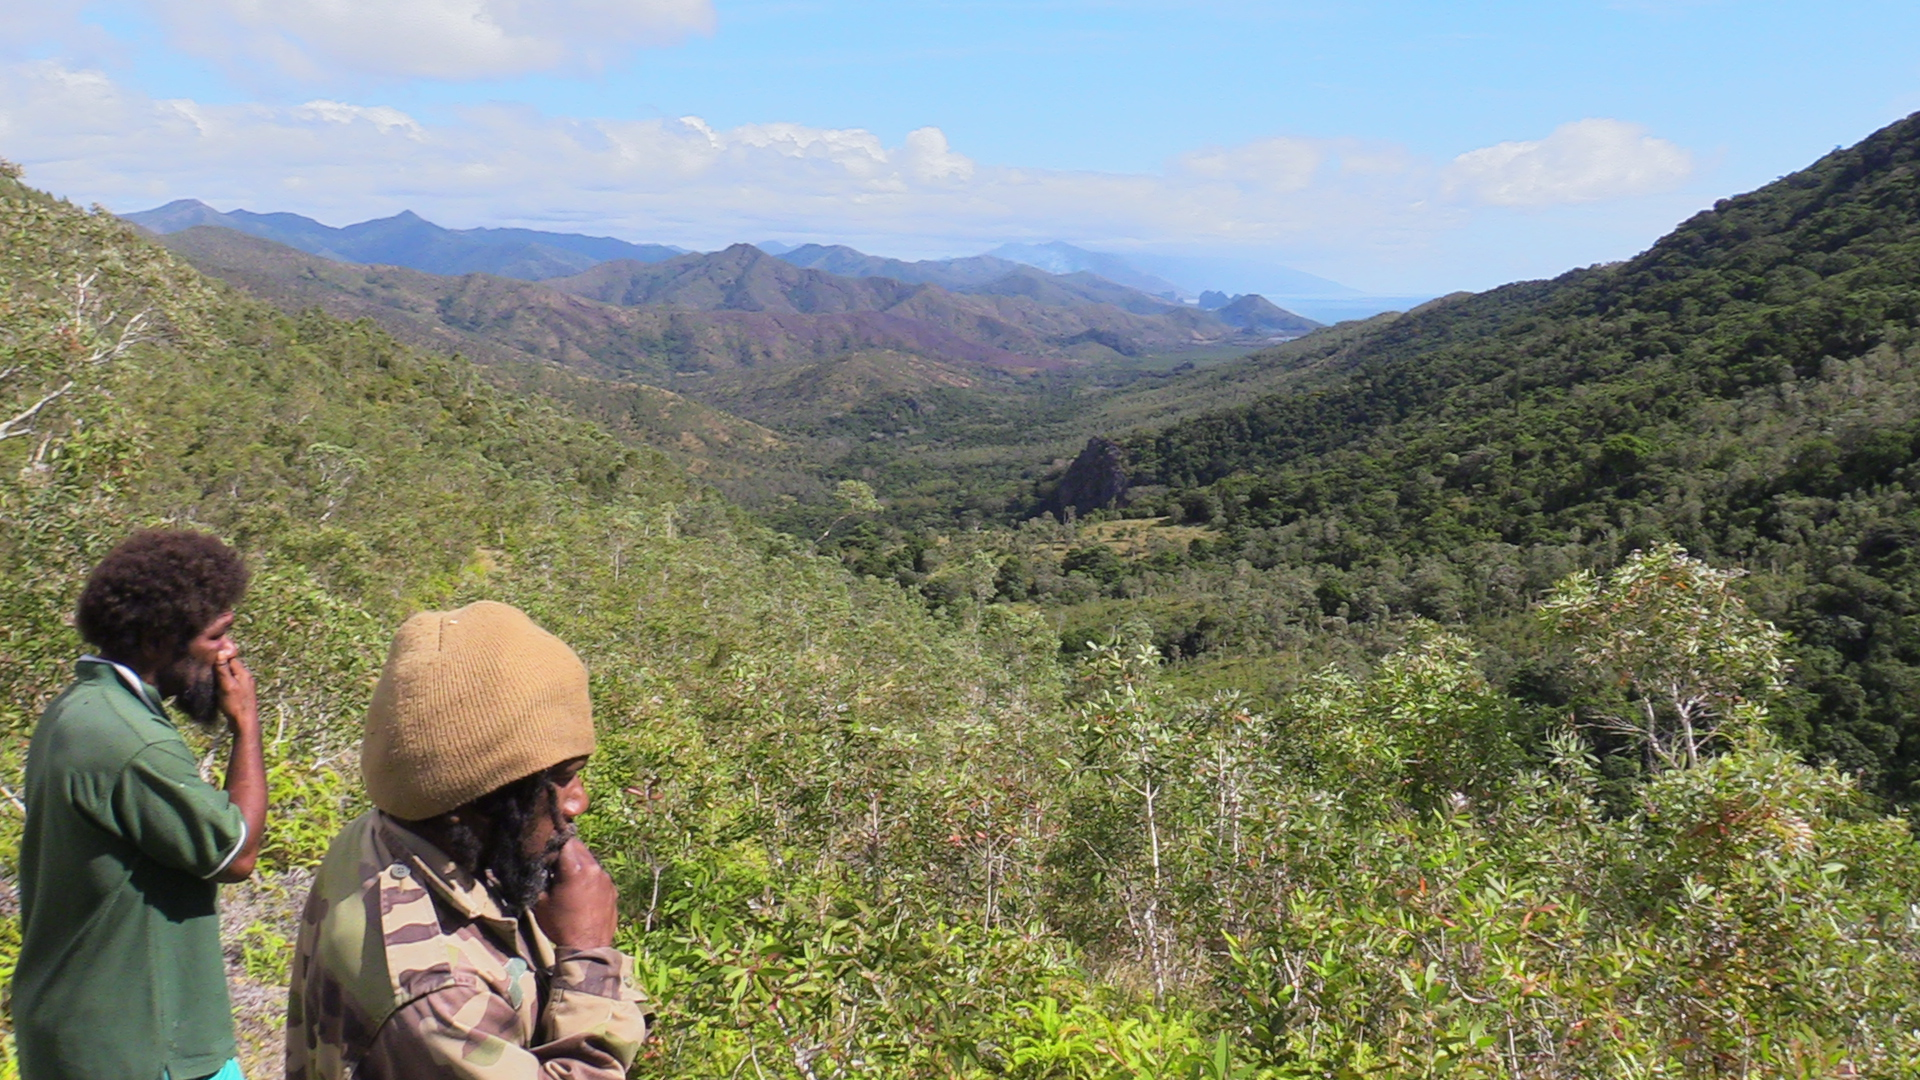
\includegraphics[width=\linewidth]{figures/koin}
	\caption{Mr. Pei and Mr. Kalène looking across the Gaheny creek unto Wanaa. Thehwaade is in the distance, and Seejanit in the blue mists beyond that.}
\end{figure}
